% ======================================================================
% GENERATED by scripts/make_master_manuscript.py from
% paper/src/ieee_access_manuscript.tex -- do not edit; edit the IEEE source
% and re-run the script. Publisher-neutral single-column version.
% ======================================================================
\documentclass[11pt]{article}

\usepackage[a4paper,top=2.5cm,bottom=2.5cm,left=2.5cm,right=2.5cm]{geometry}
\usepackage{amsmath,amssymb,amsfonts}
\usepackage{graphicx}
\usepackage{textcomp}
\usepackage[hyphens]{url}
\usepackage{bm}
\usepackage{amsthm}
\usepackage{float}
\usepackage{booktabs}
\usepackage{array}
\usepackage{rotating}
\usepackage{cite}
\usepackage[font=small,labelfont=bf,labelsep=period]{caption}
\usepackage[utf8]{inputenc}
\usepackage[T1]{fontenc}
\usepackage[hidelinks]{hyperref}
\urlstyle{same}

\renewcommand{\thetable}{\Roman{table}}
\setlength{\emergencystretch}{3em}
\graphicspath{{../../paper/figures/}}
\makeatletter\newcommand{\tabinput}[1]{\@@input #1 }\makeatother

\theoremstyle{definition}
\newtheorem{definition}{Definition}
\newtheorem{remark}{Remark}
\theoremstyle{plain}
\newtheorem{proposition}{Proposition}

\floatstyle{ruled}
\newfloat{algorithm}{tbp}{loa}
\floatname{algorithm}{Algorithm}
\newcounter{algstep}
\newenvironment{algsteps}{%
  \footnotesize
  \setcounter{algstep}{0}%
  \begin{list}{\textbf{\thealgstep:}}{%
    \usecounter{algstep}%
    \setlength{\labelwidth}{14pt}%
    \setlength{\labelsep}{4pt}%
    \setlength{\leftmargin}{20pt}%
    \setlength{\rightmargin}{0pt}%
    \setlength{\itemsep}{1pt}%
    \setlength{\parsep}{0pt}%
    \setlength{\topsep}{3pt}%
  }%
}{\end{list}}
\newcommand{\algind}[1]{\hspace*{#1.1em}}
\newcommand{\algkw}[1]{\textbf{#1}}
\newcommand{\algcomment}[1]{\textit{$\triangleright$~#1}}
\AtBeginDocument{\renewcommand{\ttdefault}{lmtt}}

\begin{document}
\begin{center}
{\Large\bfseries Lineage and Release Timing in Correlated Errors of Open-Weight Language Models: A Pair-Level Study}
\end{center}

\begin{center}
Sudharsan S$^{1}$, S.~Kanaga Suba Raja$^{1,2}$, Shree Harish V$^{1,3}$, Chin-Shiuh Shieh$^{2}$, Mong-Fong Horng$^{2}$, and Lavanya R$^{1}$
\end{center}

\vspace{0.3em}
\footnotesize
\noindent$^{1}$Department of Computer Science and Engineering, SRM Institute of Science and Technology, Tiruchirappalli 620101, India.\\
$^{2}$Research Institute of IoT Cybersecurity, Department of Electrical Engineering, National Kaohsiung University of Science and Technology, Kaohsiung 824, Taiwan, ROC.\\
$^{3}$Department of Computer Science and Engineering (Big Data Analytics), SRM Institute of Science and Technology, Tiruchirappalli 620101, India.\\
\vspace{0.3em}
Corresponding author: S.~Kanaga Suba Raja (e-mail: kanagass@srmist.edu.in).
\normalsize

\vspace{1em}
\begin{abstract}
When two open-weight language models both answer a question wrongly, how often do they choose the same wrong option, and is that more closely associated with shared ancestry or with release timing? We validated item-level predictions on the Massive Multitask Language Understanding (MMLU) benchmark for 977 models from the Open LLM Leaderboard, which form two overlapping samples that differ in how lineage is declared. In the primary sample (590 models, 173{,}755 pairs), two models descended from the same declared base model choose the same wrong option 13.3 percentage points more often than unrelated models of equal accuracy and release gap (95\% confidence interval 10.8--15.8; pairs weighted equally, so the two largest roots dominate; 28.3 points without the accuracy adjustment; mean agreement 42.3\%); in the expanded sample (928 models) the difference is 12.7 points (11.0--14.5). The association holds across twelve analyses fixed before any pairwise outcome was computed, root-level inference, item-difficulty-aware null models, a chance-adjusted agreement metric and the removal of duplicate and degenerate models. Release proximity, whether of the models themselves or of their base models, shows only small associations once accuracies are controlled, and their sign depends on the specification: same-month pairs agree up to a few points more in several specifications and less among models above 0.30 accuracy. The analysis plan and sample rules were fixed before any pairwise outcome was computed. The study is diagnostic: it does not test ensembles, and the associations are observational in a population dominated by community fine-tunes.
\end{abstract}

\noindent\textbf{Keywords:} Correlated errors, dyadic regression, error agreement, Hugging Face, large language models, model lineage, Open LLM Leaderboard.

\vspace{1em}

\section{Introduction}
\label{sec:introduction}

When several public large language models (LLMs) are asked the same hard question, they often fail together, and often in the same way. Kim~\textit{et al.}~\cite{kim2025} document this across hundreds of open and hosted models: when two models are both wrong, they choose the same wrong option far more often than chance. For anyone who combines models---a majority vote, a routing scheme, or a review step that escalates only when models disagree---this matters directly, because agreement between members is informative only if their errors are not shared~\cite{dietterich2000,kuncheva2003}.

Two explanations for shared errors compete. \emph{Lineage}: a model fine-tuned from another inherits its parameters and therefore, plausibly, its blind spots. \emph{Era}: models built in the same period draw on the same data, recipes and base models and may acquire the same mistakes without shared ancestry. The two are entangled, because a fine-tune is always released after its base. We measure era by \emph{release timing}: the month each model was uploaded to Hugging Face and, in a post-hoc analysis, the month its root base model was released.

This paper is a diagnostic study. It measures how shared wrong answers relate to lineage and release timing in a large population of open-weight models; it does not build or test ensembles, and whether the associations translate into better voting or routing is a separate question. Because shared errors are a property of \emph{pairs} of models, we model agreement on wrong answers between pairs, with lineage and release-month gap as pair-level predictors, in a design whose analysis and sample rules were fixed before any outcome was computed. Decomposing per-model accuracy into family and era variance components, the obvious alternative, is too imprecise with the few families and release quarters real populations offer (Supplementary Section~S1); an earlier version of this work attempted it, and its findings are withdrawn (Supplementary Section~S2). That attempt recorded MMLU runs for 16 of 20 planned models on a single rented GPU (one NVIDIA A100 80\,GB on RunPod) before it was stopped for budget reasons; an extraction error invalidated every per-question output, and none of its measurements is used here (Appendix; Supplementary Section~S7).

\subsection{Research Questions}
\begin{enumerate}
\item \textbf{RQ1:} Among open-weight models, is sharing a lineage root associated with choosing the same wrong answer, at equal release gap and accuracy?
\item \textbf{RQ2:} Is release proximity associated with choosing the same wrong answer, at equal lineage status and accuracy?
\end{enumerate}

\subsection{Contributions}
\begin{enumerate}
\item \textbf{A pre-specified pair-level design.} Agreement on wrong answers is modelled for pairs of models, with dyadic inference for the dependence among pairs and a simulation check of whether lineage and release timing can be separated in the population studied (Section~\ref{sec:design}).
\item \textbf{An item-level validation protocol.} For 977 leaderboard models, the correctness of each reconstructed prediction is checked item by item against the leaderboard's stored correctness flag, and two data-quality problems in the leaderboard---models listed under several names, and models that give one answer letter to almost every item---are documented and shown not to drive the results (Section~\ref{sec:data}).
\item \textbf{Evidence on the two explanations.} Shared lineage is associated with about 13 points more agreement on wrong answers; release proximity shows only small associations whose sign depends on the specification once accuracies are controlled (Section~\ref{sec:results}). Analyses run after review suggest that closer relatives agree more.
\end{enumerate}

Fig.~\ref{fig:agreement} shows the raw pattern that the study quantifies. More accurate models agree more often on their wrong answers (panel a), as Kim~\textit{et al.}~\cite{kim2025} also observe. Within the seven largest lineage roots, two models of the same root choose the same wrong option in 73.4\% of shared errors on average, against 56.4\% for two models of different roots (panel b); but roots also differ in accuracy, which is why every comparison below is made at equal accuracy. Lineage resolution, sampling, validation, the pair outcome and the pair-level model were fixed in a dated analysis plan before any pair outcome was computed (Section~\ref{sec:plan}); Fig.~\ref{fig:dataflow} gives the number of models at each step.

\begin{figure}[!htbp]
\centering
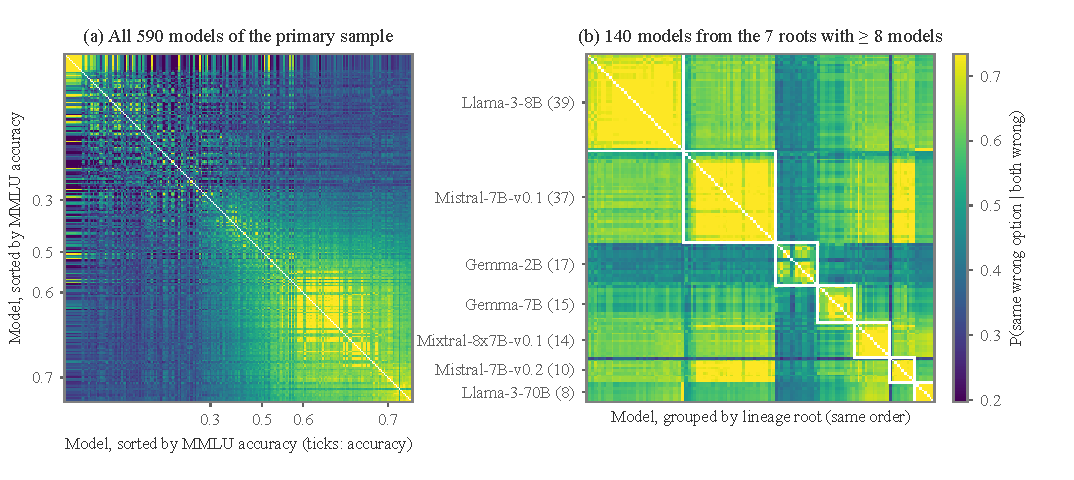
\includegraphics[width=\textwidth]{fig_agreement.pdf}
\caption{\textbf{Agreement on wrong answers between pairs of models} (primary sample; no adjustment). Each cell is the probability that the two models choose the same wrong option on the items both answer wrongly, Eq.~\eqref{eq:outcome}; the diagonal is undefined and left blank, and the color scale is clipped at the 2nd and 98th percentiles. (a) All 590 models, sorted by MMLU accuracy; tick labels give the accuracy reached at that position. (b) The 140 models of the seven roots with at least eight models, grouped by root (number of models in parentheses) and sorted by accuracy within each root; white squares enclose the same-root pairs, whose mean agreement is 0.734 against 0.564 for the different-root pairs of panel (b). Accuracy and lineage are both visible here; Section~\ref{sec:results} separates them.}
\label{fig:agreement}
\end{figure}

\section{Related Work}
\label{sec:related}

\textbf{Correlated errors in LLMs.} Kim~\textit{et al.}~\cite{kim2025} measure pairwise agreement on wrong answers across 349 Hugging Face models and 71 models from the Holistic Evaluation of Language Models (HELM) and regress it on pair characteristics, finding that a shared provider, a shared base architecture and similar size predict higher agreement, and that larger and more accurate models have more correlated errors. Their Hugging Face regressions include per-model ``generation'' covariates with small positive coefficients, and they interpret the accuracy result as newer models converging, but they do not measure how close two models' releases are or separate that from lineage, and the paper does not describe any correction for the dependence among pairs that share a model. Chen~\cite{chen2026} shows across 67 models that the gain from routing, voting or mixture-of-agents is capped by the rate at which all models fail the same query. Kuai~\textit{et al.}~\cite{kuai2026} audit 18 models from six families for synchronized failures and reweight verifier ensembles accordingly. Goel~\textit{et al.}~\cite{goel2025} propose chance-adjusted probabilistic agreement (CAPA), a similarity metric based on overlapping mistakes, and report that mistakes become more similar as capability increases. Kim~\cite{kimd2026} audits majority-vote gain across subsets of 30 models and finds that, once capability is controlled, shared errors are the only stable predictor of lower gain. In vision-language models, Bugaud~\cite{bugaud2026} finds correlated mistakes within architectural families and proposes family-aware aggregation. Evidence on families is not uniform: across 20 open-weight models from 10 families, Li and Hai~\cite{lihai2026} do not detect an association between same-family membership and error dependence once capability is controlled (the interval includes zero), and Hossain~\textit{et al.}~\cite{hossain2026} report, for four base models from three families, that overlap in one class of errors tracks shared pretraining recency more than architectural lineage, which they describe as suggestive. In both, ``family'' groups separately pretrained models; in our data, related models share a checkpoint. Tieman and Markou~\cite{tieman2026} show that diversity in how models generate outputs predicts lower correlated failure.

\textbf{Null models for excess agreement.} Jo, Garg and Raghavan~\cite{jo2026} show that whether models agree ``more than expected'' depends on the null model of independence---accounting for item difficulty changes conclusions---and on the population of models and items. Paquin and Jain~\cite{paquin2026} fit item response models to 1{,}000 open-weight models on the same 14{,}042 MMLU items and show that item difficulty follows different structures in STEM and non-STEM subjects; they study what the aggregate score measures, not whether two models fail in the same way, so their population and items overlap ours but their question does not. Three estimands are in use: correlated correctness (whether two models fail the same items), conditional agreement on the wrong option (whether two models that both fail choose the same distractor~\cite{kim2025}) and accuracy-adjusted similarity~\cite{goel2025}. Our primary estimand is the second and our secondary the first. Our quantity of interest is a \emph{contrast} between related and unrelated pairs rather than the level of excess agreement, so a null that shifts all pairs equally leaves it unchanged; we test this with item-difficulty-aware nulls.

\textbf{Lineage and ancestry.} Laufer, Oderinwale and Kleinberg~\cite{laufer2025} map the family trees of about 1.86 million Hugging Face models from declared parents and study how metadata traits are inherited. Horwitz, Shul and Hoshen~\cite{horwitz2025} recover model trees from weights, and Wu~\textit{et al.}~\cite{wu2026dna} infer relationships from a compact representation of model behaviour. Tamura~\textit{et al.}~\cite{tamura2025} show that declared parent--child relations improve the prediction of benchmark performance, and Choi~\textit{et al.}~\cite{choi2026} find that attention-head truthfulness scores are preserved from base models to their descendants. Nikoli\'c~\textit{et al.}~\cite{nikolic2025} test whether one model is derived from another from output similarity alone. PhyloLM~\cite{phylolm2024} reconstructs phylogenies from output similarity, and Li~\textit{et al.}~\cite{li2026roots} trace the lineage of post-training datasets. None of these measures whether related models make the same errors, item by item.

\textbf{Statistical tools.} Crossed variance-component models estimated by restricted maximum likelihood (REML)~\cite{patterson1971,harville1977,searle1992} and generalizability theory~\cite{brennan2001} underlie the per-model analysis in Supplementary Section~S1; Messing~\cite{messing2026} shows that ignoring design choices in LLM pipelines understates evaluation uncertainty. Pairwise outcomes are dependent, because every model appears in many pairs; we use dyadic cluster-robust variance estimators~\cite{fafchamps2007,cameron2011,aronow2015} and a delete-one-root jackknife~\cite{efron1982}. Ensemble gains depend on error diversity~\cite{breiman2001}, and monoculture arguments~\cite{kleinberg2021,bommasani2022} treat correlated error as a risk.

\textbf{Our contribution.} We do not claim to be the first study of correlated errors in LLMs. Relative to Kim~\textit{et al.}~\cite{kim2025}, the closest work, the outcome is the same, but lineage is resolved per model from declared fine-tune ancestry rather than coded as shared provider or architecture, release timing is tested jointly with it at equal accuracy, and inference allows for the dependence among pairs. To our knowledge this is the first study to examine declared ancestry and release proximity jointly as correlates of agreement on wrong answers. Table~\ref{tab:prior} summarizes the differences.

\begin{table}[!htbp]
\caption{\textbf{Relation to the closest prior work.}}
\label{tab:prior}
\centering
\footnotesize
\resizebox{\ifdim\width>\textwidth\textwidth\else\width\fi}{!}{\begin{tabular}{p{0.15\textwidth}p{0.26\textwidth}p{0.24\textwidth}p{0.25\textwidth}}
\toprule
Study & Outcome & Relatedness of models & Release timing \\
\midrule
Kim \textit{et al.}~\cite{kim2025} & Same wrong option when both wrong & Shared provider, base architecture & Per-model generation covariate; proximity not tested \\
Goel \textit{et al.}~\cite{goel2025} & Chance-adjusted agreement (CAPA) & -- & Capability, not time \\
Chen~\cite{chen2026} & Rate at which all models fail an item & -- & -- \\
Kuai \textit{et al.}~\cite{kuai2026} & Synchronized failures of LLM judges & Model family & -- \\
Jo \textit{et al.}~\cite{jo2026} & Excess agreement under alternative nulls & -- & -- \\
Kim~\cite{kimd2026} & Majority-vote gain of ensembles & -- & Capability controlled, not time \\
Li and Hai~\cite{lihai2026} & Error dependence in voting committees & Model family (separately pretrained) & -- \\
Hossain \textit{et al.}~\cite{hossain2026} & Overlap of temporal-conflict errors & Architecture lineage & Pretraining recency (four models) \\
Bugaud~\cite{bugaud2026} & Correlated mistakes of vision-language models & Architecture family & -- \\
PhyloLM~\cite{phylolm2024}, LLM DNA~\cite{wu2026dna} & Output similarity used to infer relations & Inferred from outputs & -- \\
This study & Same wrong option when both wrong; phi; CAPA & Declared ancestry: shared root, tree distance & Upload and root release months, jointly with lineage \\
\bottomrule
\end{tabular}}
\end{table}

\section{Data and Lineage}
\label{sec:data}

\subsection{Source and Validation}
The first version of the Open LLM Leaderboard~\cite{beeching2023} evaluated thousands of open-weight models on MMLU~\cite{hendrycks2021} (5-shot) with the LM Evaluation Harness~\cite{gao2021} and published per-item details, including per-option log-likelihoods. For each model we select the most complete run covering all 57 subjects and read, per item, the per-option log-likelihoods, the correct option, the leaderboard's stored correctness and, where present, an item hash. A model is accepted only if (i) all 14{,}042 items are present, (ii) the correctness status (correct or incorrect) of the option with the highest log-likelihood matches the leaderboard's stored item-level correctness flag on \emph{every} item, and (iii) item order and correct options match a reference model. Check (ii) is the decisive one: an earlier version of this work recorded the first answer option for every item, producing constant predictions that no aggregate statistic flagged (Supplementary Section~S2), and that error, a misaligned item order and a misread answer key each produce thousands of disagreements. Because the stored flag records only whether an answer was correct, check (ii) validates correctness status; it does not independently verify which wrong option a model chose, which is read from the leaderboard's own per-option log-likelihoods. Item order and answer keys are checked separately, by (iii) and by the answer-key test below. The protocol also cannot detect an error in the leaderboard's own evaluation, such as an unsuitable prompt format for a particular model. For one spot-checked model (Llama-2-7b-hf), extracted accuracy also equals the leaderboard's official aggregate (43.80). Three storage layouts occur among the accepted models (692 in the newest layout, 253 and 32 in two older ones). In the newest the correct-option column is blank and the correct option is taken from the reference model by position, which check (ii) then validates: a misaligned answer key fails on roughly three quarters of items. We keep each model's chosen option per item; the per-option scores serve only for validation.

\subsection{Lineage and Release Timing}
\label{sec:lineage}
Lineage is resolved by following each model's declared \texttt{base\_model} on Hugging Face to a \emph{root}, collapsing repository renames and a documented list of straight re-uploads and quantisations. A chain is unresolved if it passes through a merge, reaches a deleted ancestor, or ends at a fine-tune with no declared parent. Supplementary Section~S8 gives the exact rules as an algorithm. Two populations are defined: \emph{primary}, in which every link comes from a model card, and \emph{expanded}, which also accepts a model's own first link from the \texttt{\_name\_or\_path} field of its configuration file when that field names an existing repository. A \emph{strict} variant of each keeps only chains ending at a checkpoint the leaderboard lists as pretrained.


Declared lineage is sparse. Of the 6{,}896 models on the leaderboard, 721 are eligible for the primary population. The reasons for exclusion overlap: 4{,}843 models declare no parent, 1{,}637 are merges and 776 more descend through one, 1{,}209 are no longer on the Hub, 385 are adapter or delta weights, 339 chains end at a fine-tune with no declared parent, and 56 reach a deleted ancestor. For the 2{,}978 models excluded only for lacking a declared parent, the configuration file names an existing repository in 1{,}073 cases; in the others it names a local path (838), a string that is not a repository identifier (353), the model itself (228), a repository that no longer exists (111) or a merge tool (63), or the field or file is missing (312). Of the 1{,}073, 574 resolve to an eligible root and join the expanded population (1{,}295 models). \emph{Upload month} is the Hub creation month of a model's repository (27 months, March 2022 to July 2024); \emph{root release month} is that of its root.

\subsection{Samples}
Each population was sampled with at most 40 models per root and a fixed seed, and the samples were frozen with SHA-256 hashes before any prediction was downloaded (Fig.~\ref{fig:dataflow}). Of the 1{,}018 models in the two overlapping samples, 977 passed validation; 41 were excluded and logged, and none was replaced. The analysed primary sample has 590 models from 351 roots (63 with two or more models) and 173{,}755 pairs; the expanded sample has 928 models from 422 roots (108) and 430{,}128 pairs. The largest roots are Llama-3-8B and Mistral-7B-v0.1 (39 and 37 primary models). Median accuracy is 0.415, and 247 primary models score below 0.30, close to chance for four options. Table~\ref{tab:desc} describes the four analysed samples.

\begin{table}[!htbp]
\caption{\textbf{Analysed samples.} S2: models with accuracy $\geq 0.30$. Agreement: probability of the same wrong option when both models are wrong, Eq.~\eqref{eq:outcome}.}
\label{tab:desc}
\centering
\footnotesize
\setlength{\tabcolsep}{2.5pt}
\resizebox{\ifdim\width>\textwidth\textwidth\else\width\fi}{!}{%
\begin{tabular}{lcccc}
\toprule
 & Primary & Primary, S2 & Expanded & Expanded, S2 \\
\midrule
\tabinput{../../paper/tables/tab_descriptives.tex}
\bottomrule
\end{tabular}}
\end{table}

\begin{figure}[!htbp]
\centering
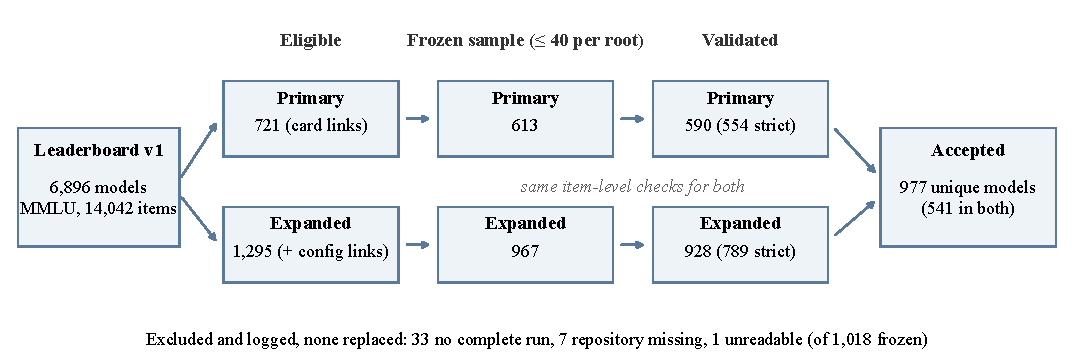
\includegraphics[width=\textwidth]{fig_dataflow.pdf}
\caption{\textbf{Study flow.} \emph{Data collection}: lineage is resolved for every leaderboard model, the two samples are drawn and frozen, and each downloaded model is validated item by item. \emph{Pair-level analysis}: solid boxes were fixed in the dated plan and amendments before any pair outcome was computed; dashed boxes were partly added after the first results (Table~\ref{tab:status}). The primary population accepts only lineage links declared on model cards; the expanded population also accepts a model's first link from its configuration file. The two frozen samples overlap, so the 977 accepted models are counted once. Strict: root verified as a pretrained checkpoint. Item-level checks, identical for both samples: all 14,042 items present; the correctness status of the highest-scoring option matches the stored item-level correctness flag on every item (this validates correctness, not the specific wrong option chosen); item order and correct options match a reference model. Excluded models were logged and not replaced.}
\label{fig:dataflow}
\end{figure}

\subsection{Data Quality}
Two problems in the leaderboard data affect pairwise analyses. First, some models are listed more than once, a redundancy also noted by Paquin and Jain~\cite{paquin2026}: in the primary sample, 50 leaderboard entries resolve on the Hub to only 23 repositories (renamed or moved), and most such pairs give identical predictions on every item; 193 primary pairs agree on at least 99.9\% of items. Second, 21 primary models choose one answer letter on at least 95\% of items; all score below 0.30. Both inflate agreement for some pairs, in opposite directions for the lineage contrast. Neither was anticipated in the analysis plan; Section~\ref{sec:robust} reports the results without them.

\subsection{How Lineage and Release Timing Overlap}
Fig.~\ref{fig:lineagemap} places the primary models on a grid of root by upload month and shows what the data can identify. Most roots contribute one model (288 of 351); such models enter only different-root pairs, so the lineage contrast is identified by the 63 roots with two or more models. The fine-tunes of a root are uploaded within a few months of one another, so same-root pairs are concentrated at short gaps (711, 1{,}004, 259, 45 and 1 pairs at 0, 1--2, 3--5, 6--11 and 12 or more months), and gaps of a year or more are populated almost entirely by different-root pairs.

\begin{figure}[!htbp]
\centering
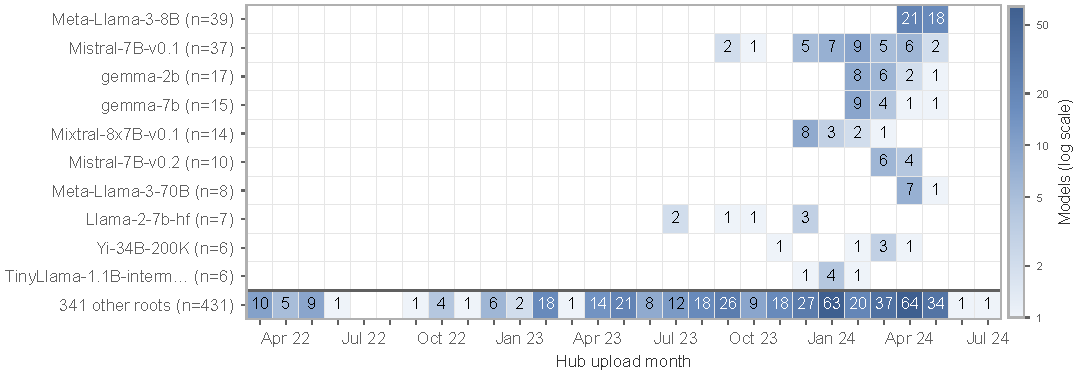
\includegraphics[width=\textwidth]{fig_lineage_month_map.pdf}
\caption{\textbf{Lineage roots by upload month} (primary sample, 590 models). Each cell counts the models of one root uploaded in one month (log color scale); the marginal bars give the models per month (top, split into the ten largest roots and the rest) and per row (right, log scale). The 10 largest roots are shown individually; the bottom row pools the other 341 roots, most of which contribute one model. Fine-tunes of a root cluster within a few months, so same-root pairs occur mainly at short release gaps.}
\label{fig:lineagemap}
\end{figure}

\section{Study Design}
\label{sec:design}

Fig.~\ref{fig:dataflow} summarizes the study from source data to checks, and which steps were fixed before any pair outcome was computed.

\subsection{Why Pairs Rather Than Models}
The natural first design treats each model's accuracy as the outcome and decomposes its variance into a family component and a release-era component with a crossed random-effects model. The components are identified in our populations, but they cannot be estimated precisely. Supplementary Fig.~S1 shows the worst-case Monte Carlo root-mean-square error (RMSE) of either variance share across four scenarios: designs with five to seven families, as real populations of pretrained bases provide, have an RMSE of at least 0.18, and bringing both shares within 0.10 requires about 60 families and 14 release quarters (Supplementary Section~S1). The traits in that analysis are simulated on each design's structure; the design labelled 16 takes only the family and quarter labels of the 16 models run in the earlier per-model evaluation, not their measured accuracies. The constraint is the number of levels of each factor, which more models do not supply. Pairs avoid it: shared errors are a pair-level quantity, lineage and release gap are pair-level attributes, and 590 models yield 173{,}755 pairs whose comparisons span every combination of lineage status and gap that the data contain.


\subsection{Outcome}
For models $i$ and $j$, let $c_{ik}$ be model $i$'s chosen option on item $k$ and $t_k$ the correct option. The outcome is the conditional agreement~\cite{kim2025}
\begin{equation}
a_{ij} = \frac{\sum_k \mathbf{1}[c_{ik} = c_{jk} \neq t_k]}{\sum_k \mathbf{1}[c_{ik} \neq t_k]\,\mathbf{1}[c_{jk} \neq t_k]},
\label{eq:outcome}
\end{equation}
the probability of choosing the same wrong option given that both are wrong. Every pair contributes all items on which both models are wrong: between 1{,}166 and 10{,}820 items (median 4{,}109). Each item has three wrong options, so two models choosing among them independently and uniformly would give $a_{ij} = 1/3$. The outcome measures \emph{how} two models fail when they both fail; \emph{whether} they fail on the same items is measured by the secondary outcome, the phi coefficient of their error indicators.

\subsection{Pair Model}
The pre-specified model is
\begin{equation}
\begin{aligned}
a_{ij} = {}& b_0 + b_L\, s_{ij} + \textstyle\sum_{h} b_{E,h}\, \mathbf{1}[\,|m_i - m_j| \in h\,]\\
& + \gamma_1 (\mathrm{acc}_i + \mathrm{acc}_j) + \gamma_2 |\mathrm{acc}_i - \mathrm{acc}_j| + \varepsilon_{ij},
\end{aligned}
\label{eq:pair}
\end{equation}
estimated by ordinary least squares (OLS), where $s_{ij}$ indicates a shared lineage root, $m_i$ is the upload month, and $h$ ranges over gap bins of 0, 1--2, 3--5 and 6--11 months, with 12 or more months as reference. We call $b_L$ the \emph{shared-root coefficient} and $b_{E,0}$ the \emph{same-month coefficient}: the difference in agreement between pairs uploaded in the same month and pairs uploaded 12 or more months apart, at equal lineage status and accuracies. Coefficients are differences in probability; in the text we report them in percentage points. Both are conditional associations, not causal effects. Fig.~\ref{fig:schematic} illustrates the two predictors: every pair carries one value of each, so same-root pairs occur at several gaps and same-month pairs occur with and without a shared root.

\begin{figure}[!htbp]
\centering
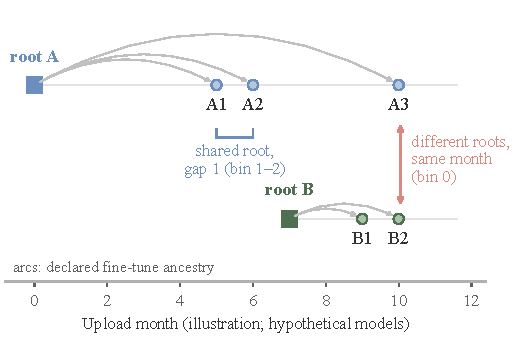
\includegraphics[width=0.65\textwidth]{fig_schematic.pdf}
\caption{\textbf{The two pair-level predictors} (hypothetical models). Squares are lineage roots, circles fine-tunes at their upload month; arcs show declared ancestry. A1 and A2 share a root and were uploaded one month apart (gap bin 1--2); A3 and B2 have different roots but the same upload month (gap bin 0).}
\label{fig:schematic}
\end{figure}

The accuracy terms are pre-specified because two models of similar accuracy tend to fail on similar items, and the items strong models fail are the hardest, which may have more attractive distractors. They are not neutral: if lineage or release timing affects agreement partly through accuracy, adjustment removes that part, so we also report the model without them.

\subsection{Secondary Outcomes and Null Models}
\label{sec:defs}
Five further quantities are used, each as the outcome of Eq.~\eqref{eq:pair} in place of $a_{ij}$. With $w_{ik} = \mathbf{1}[c_{ik} \neq t_k]$ the error indicator of model $i$ on item $k$:
\begin{itemize}
\item \emph{Phi coefficient} (pre-specified secondary): the Pearson correlation of $w_{ik}$ and $w_{jk}$ over items, which measures whether two models fail the same items.
\item \emph{Option-distribution chance} (exploratory): $a_{ij}$ minus $\sum_o \omega_i(o)\,\omega_j(o)$, where $\omega_i(o)$ is the share of model $i$'s wrong answers that are option $o$; it removes agreement expected from two models' preferences for answer letters.
\item \emph{CAPA from chosen options} (post hoc): $\kappa_{ij} = (o_{ij} - e_{ij})/(1 - e_{ij})$, with $o_{ij}$ the share of items on which the two choose the same option and
\[ e_{ij} = \mathrm{acc}_i\,\mathrm{acc}_j + (1-\mathrm{acc}_i)(1-\mathrm{acc}_j)/3, \]
after Goel~\textit{et al.}~\cite{goel2025}; the original uses option probabilities, which we did not retain.
\item \emph{Distractor null N1} (post hoc): $a_{ij} - \overline{q}_{ij}$, where $q_k = \sum_o p_k(o)^2$, $p_k(o)$ is the share of wrong models choosing wrong option $o$ on item $k$, and $\overline{q}_{ij}$ averages $q_k$ over the pair's jointly wrong items. N1a computes $p_k$ from all models; N1b weights every root equally, so that a large family does not define the null.
\item \emph{Rasch null N2} (post hoc): $\frac{1}{K}\sum_k (w_{ik}w_{jk} - \hat P_{ik}\hat P_{jk})$, where $\operatorname{logit} \hat P_{ik} = \hat d_k - \hat\theta_i$ is fitted by joint maximum likelihood; it measures co-failure beyond what item difficulty and model ability predict.
\end{itemize}
The S1 covariate is defined in Section~\ref{sec:plan}. For release timing we also report, post hoc, an \emph{equivalence bound}: the largest absolute same-month coefficient not excluded by its 90\% jackknife interval.

\subsection{Inference}
Every model enters many pairs, so pair residuals are dependent. The pre-specified standard errors (SEs) are dyadic cluster-robust~\cite{fafchamps2007,cameron2011,aronow2015}: with $\mathbf{x}_p$ the covariates and $\hat e_p$ the residual of pair $p$,
\begin{equation}
\widehat{V}(\hat{\mathbf{b}}) = (X^\top X)^{-1}\Big(\sum_{p,q:\;p \cap q \neq \emptyset} \hat e_p \hat e_q\, \mathbf{x}_p \mathbf{x}_q^\top\Big)(X^\top X)^{-1},
\label{eq:dyadic}
\end{equation}
where $p \cap q \neq \emptyset$ means that pairs $p$ and $q$ share a model (including $p = q$). Because fine-tunes of one root may err alike beyond what sharing a model captures, we also use two procedures that treat the root as the unit of dependence: root-level dyadic clustering (Eq.~\eqref{eq:dyadic} with ``share a root'') and a delete-one-root jackknife, which refits the model $G$ times, omitting every pair that involves one of the $G$ roots, and estimates the variance as $\frac{G-1}{G}\sum_{r} (\hat{\mathbf{b}}_{(r)} - \bar{\mathbf{b}})^2$. The jackknife gives the widest intervals for both coefficients in every sample, so we report it as the main interval.

\subsection{Analysis Plan and Deviations}
\label{sec:plan}
The plan, written before any pair outcome was computed, fixed the outcome, Eq.~\eqref{eq:pair}, the model-level SEs, the phi outcome as secondary, a tree-distance lineage predictor as secondary, the sample rules and a simulation check (Section~\ref{sec:gate}). Three dated amendments followed, each before the quantities it concerns were computed: (1) the source moved from the second to the first version of the leaderboard, whose item-level files are not access-gated; (2) the populations were defined as above and the cap was set to 40 models per root; (3) after the accuracies of the first 443 validated models showed many near-chance models, two sensitivity analyses were added: \emph{S1} adds the total-variation distance $\tfrac12\sum_{o}|\pi_i(o) - \pi_j(o)|$ between the two models' distributions $\pi$ over chosen answer options as a covariate, because two models favouring the same letters agree more for that reason alone, and \emph{S2} keeps models with accuracy at least 0.30. Amendment~3 is the one decision informed by data, though by per-model accuracies rather than pair outcomes. The plan, the three amendments and the first pair outcome were all committed on 9 October 2026, within about four and a half hours; the order is recorded only by the repository's commit times. An earlier paragraph of the same plan document, written an hour before the fixed specification, proposed crossed random effects for the pair model; the specification marked as fixed before data (OLS with dyadic SEs) is the one used. The plan was not deposited with an independent registry, so we call it pre-specified rather than pre-registered. Table~\ref{tab:status} gives the status of every analysis, including planned analyses that were not run.

\begin{table}[!htbp]
\caption{\textbf{Status of each analysis.} Pre-spec.: in the analysis plan. Amend.: dated amendment before any pair outcome. Explor.: not in the plan, run with or after the pre-specified analyses. Post hoc: added in response to review. Plan; run after review: specified in the analysis plan but first run after the main results were known. WLS: weighted least squares; CAPA: chance-adjusted agreement.}
\label{tab:status}
\centering
\footnotesize
\setlength{\tabcolsep}{3pt}
\resizebox{\ifdim\width>\textwidth\textwidth\else\width\fi}{!}{\begin{tabular}{p{0.6\textwidth}l}
\toprule
Analysis & Status \\
\midrule
Pair model, Eq.~\eqref{eq:pair}; model-level dyadic SEs; phi outcome & Pre-spec. \\
Simulation check and its criteria & Pre-spec. \\
Leaderboard version~1; populations; cap of 40 & Amend.~1--2 \\
S1 (option distribution), S2 (accuracy $\geq 0.30$) & Amend.~3 \\
Root-level SEs; WLS; option-chance outcome; size controls & Explor. \\
Without accuracy terms; item-difficulty nulls; CAPA & Post hoc \\
Root release month; equivalence bound; duplicate, degenerate and config checks & Post hoc \\
500-replicate simulation audit; cap-15 subset & Post hoc \\
Heterogeneity by root, capability and subject; lineage detection & Post hoc \\
Tree-distance predictor & Plan; run after review \\
Flexible accuracy control; within-root dose-response; item fixed effects; root bootstrap and permutation; real-accuracy simulation; MMLU-Redux & Post hoc \\
Replication on leaderboard version~2 (access-gated) & Not done \\
Per-model accuracy decomposition on the leaderboard population; same-root-organisation predictor & Not done \\
\bottomrule
\end{tabular}}
\end{table}

\subsection{Simulation Check}
\label{sec:gate}
Because same-root pairs are concentrated at short gaps (Fig.~\ref{fig:lineagemap}), a release-time effect could leak into the lineage coefficient or vice versa. Before any pair outcome was computed, we simulated item-level choices on the actual roster. Each model answers correctly with probability $\operatorname{logit}^{-1}(\theta_i - d_k)$, with $\theta_i \sim \mathcal{N}(0.3, 1)$ and $d_k \sim \mathcal{N}(0, 1)$; when wrong, it picks a root-specific preferred option with probability $\lambda_L$, a month-specific preferred option (persisting from month to month with probability 0.8) with probability $\lambda_E$, an option preferred by all models with probability $\lambda_A = 0.15$, and otherwise a uniform wrong option. Eq.~\eqref{eq:pair} with dyadic SEs was refitted to each simulated data set. The criteria were: false rejection under no effect at most 10\%; \emph{leakage}, the rejection rate of the wrong coefficient under a single true effect, at most 10\%; and power at least 80\% at $\lambda = 0.05$. With 20 replicates per scenario, the cap of 40 met all three. With 20 replicates, rejection rates move in steps of five points, so after the results were known we repeated the check with 500 replicates per scenario (Supplementary Section~S3, with figure and tables). The null and power criteria are met: false rejection is 5.8--7.8\% for the chosen design, and power at $\lambda = 0.05$ is 100\% for both coefficients. Leakage into the lineage coefficient is 10.8\% (95\% CI 8.4--13.8) at the strongest release-time effect, $\lambda_E = 0.10$, and 12.6\% in the expanded design, against the 10\% criterion; every other leakage rate lies between 3.6 and 7.8\%. The leak is a small positive bias: the simulated lineage estimate averages $1.41 \times 10^{-4}$ although its true value is zero (Monte Carlo SE $0.13 \times 10^{-4}$; $1.39 \times 10^{-4}$, SE $0.18 \times 10^{-4}$, relative to the no-effect scenario), about 2\% of the simulated same-month coefficient at $\lambda_E = 0.10$ ($6.45 \times 10^{-3}$). Extrapolating that ratio to the largest observed same-month coefficient implies a bias of about $3 \times 10^{-4}$ on an estimate of 0.133; this is an extrapolation, not a measured bias of the main estimate. The audit also found the model-level SEs 3--5\% smaller than the simulated spread of the estimates in the primary design, one reason we report root-level intervals. It ranked the caps differently from the 20-replicate check, under which caps of 15 and none had failed; cap 40 remains the primary design because it was the dated choice.

Both checks drew abilities independently of root and month, whereas in the data accuracy clusters within roots and upload months. A second post-hoc re-run sets each simulated model's ability so that its expected accuracy equals its observed accuracy (200 replicates per scenario; Supplementary Section~S6). False rejection under no effect is then 5.0\% for the shared-root coefficient and 8.5\% for the same-month coefficient, and leakage into the lineage coefficient is at most 7.5\%, within the 10\% criterion. A further scenario with no lineage or release-time effect, in which the probability of choosing a common distractor rises with ability, exposes the cost of the linear accuracy control: the shared-root coefficient is rejected in 27\% of replicates and the 1--2-month coefficient in 31\%, although the induced bias is small ($-0.15$ points for lineage, against the lineage hypothesis). Decile accuracy cells reduce the shared-root false rejection to 9\% but leave 16\% for the same-month coefficient. In the data, flexible accuracy controls move the lineage estimate by at most 1.5 points (Section~\ref{sec:robust}).


\section{Results}
\label{sec:results}

\subsection{The Raw Pattern}
Fig.~\ref{fig:gap} shows the finding before any modelling. At every release gap at which both kinds of pair occur, same-root pairs choose the same wrong option on 71--75\% of jointly wrong items and different-root pairs on 40--45\% (overall 73.1\% and 42.0\%, mean 42.3\%). Among different-root pairs, agreement declines slowly with the gap, from 0.45 in the same month to 0.37 at a year or more. Kim~\textit{et al.} report the same mean for a later leaderboard snapshot~\cite{kim2025}, but on a different question set with mostly ten answer options, so the coincidence is not evidence of validity.

\begin{figure}[!htbp]
\centering
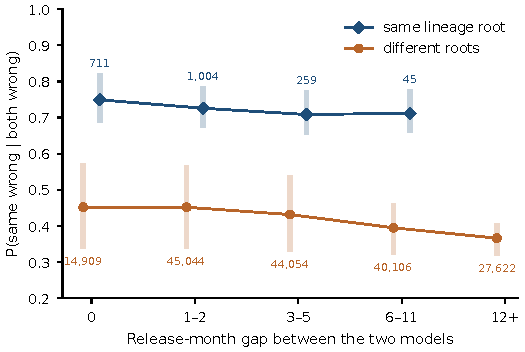
\includegraphics[width=0.65\textwidth]{exp04_agreement_by_gap.pdf}
\caption{\textbf{Agreement on wrong answers by release-month gap} (primary sample, no adjustment). Half-violins: kernel density of $a_{ij}$ across pairs (left, different roots; right, same root), scaled to equal height within each half; markers and lines: means; bars: interquartile ranges, not confidence intervals; labels: number of pairs. Dashed line: 1/3, the agreement if both models chose uniformly among the three wrong options, a descriptive reference only (the item-difficulty-aware nulls are in Section~\ref{sec:robust}). Bins with fewer than 20 pairs are omitted.}
\label{fig:gap}
\end{figure}

\subsection{Primary Result and Pre-Specified Analyses}
In the primary analysis, sharing a lineage root is associated with a 13.3-point higher probability of choosing the same wrong option (jackknife 95\% CI 10.8--15.8; model-level CI 11.8--14.8). Two models uploaded in the same month agree 0.4 points more than two uploaded a year or more apart (jackknife CI $-0.5$ to $+1.3$). Across the twelve analyses fixed before any pair outcome was computed (Table~\ref{tab:prereg}, Fig.~\ref{fig:forest}; the populations, the cap and S1--S2 come from dated amendments, Table~\ref{tab:status}) the shared-root coefficient ranges from 11.7 to 13.4 points. The estimate weights every pair equally, so roots contribute in proportion to their number of same-root pairs; Section~\ref{sec:hetero} reports estimates that count each root once. The same-month coefficient is positive when the answer-option distribution is controlled (S1: $+1.0$, CI $+0.05$ to $+1.95$) and negative among models above 0.30 accuracy (S2: $-1.5$, model-level CI $-2.7$ to $-0.2$, jackknife CI $-3.0$ to $+0.1$): its sign is not stable. The other gap bins show the same pattern. In raw terms, before any adjustment, when two fine-tunes of one base model both fail an item they pick the same distractor about three times in four, and two unrelated models about two times in five; part of that raw gap reflects accuracy, and the adjusted difference at equal accuracy and release gap is the 13.3 points above.

\begin{table}[!htbp]
\caption{\textbf{Analyses fixed before any pair outcome} (analysis plan and its dated amendments, Table~\ref{tab:status}). Coefficients of Eq.~\eqref{eq:pair} with 95\% CIs from model-level dyadic SEs; same month is the 0-month gap bin relative to 12 or more months, and $p$ refers to it. Strict: root verified as pretrained; S1: answer-option-distribution covariate; S2: models with accuracy $\geq 0.30$.}
\label{tab:prereg}
\centering
\footnotesize
\resizebox{\ifdim\width>\textwidth\textwidth\else\width\fi}{!}{\begin{tabular}{lrrccc}
\toprule
Analysis & Models & Pairs & Shared root & Same month & $p$ (same month) \\
\midrule
\tabinput{../../paper/tables/tab_prereg.tex}
\bottomrule
\end{tabular}}
\end{table}

\begin{figure}[!htbp]
\centering
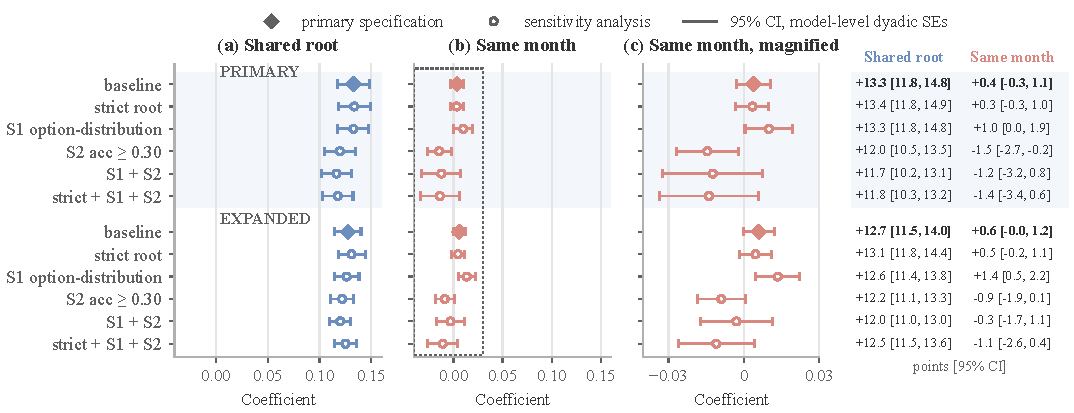
\includegraphics[width=\textwidth]{exp04_forest.pdf}
\caption{\textbf{Shared-root and same-month coefficients in the twelve analyses fixed before any pair outcome} (95\% CIs, model-level dyadic SEs). Panels (a) and (b) share one horizontal scale, so the sizes of the two associations can be compared; panel (c) magnifies the dotted region of (b) on its own scale, so that the sign changes of the same-month coefficient across specifications are visible. Diamonds: the primary specification of each population. The right-hand column gives each coefficient and interval in points. These model-level intervals allow a like-for-like comparison across the twelve analyses; they are narrower than the delete-one-root jackknife interval reported for the headline estimate (10.8--15.8 points; Fig.~\ref{fig:inference}).}
\label{fig:forest}
\end{figure}

\subsection{Adjusting for Accuracy}
Accuracy can mediate both associations: fine-tunes of one root tend to have similar accuracies, and so do models of one period. Accuracy rose steeply over the period (Fig.~\ref{fig:accuracy}): the median primary model scores 0.26 among models uploaded in 2022--2023 and 0.59 among those uploaded in 2024 (Spearman correlation with upload month 0.41), and models of similar accuracy agree more (in the pre-specified model, agreement rises with the accuracy sum and falls with the accuracy difference). Without the accuracy terms (Fig.~\ref{fig:rawadj}), the shared-root coefficient is 28.3 points and the release-gap coefficients are graded, from 8.7 points in the same month to 2.9 at 6--11 months. With them, the shared-root coefficient is 13.3 points and every release-gap coefficient is within 0.6 points of zero in both populations. If accuracy is a mediator, the unadjusted coefficients are total associations and the adjusted ones the part not running through accuracy; if accuracy and the predictor share a cause, adjustment removes a confounded component. The data cannot distinguish these readings. Under either, the predictors differ in the same way: once both accuracies are known, release proximity adds nothing of stable sign in the pre-specified model, while a shared root still adds about 13 points (Section~\ref{sec:robust} examines finer accuracy controls).

\begin{figure}[!htbp]
\centering
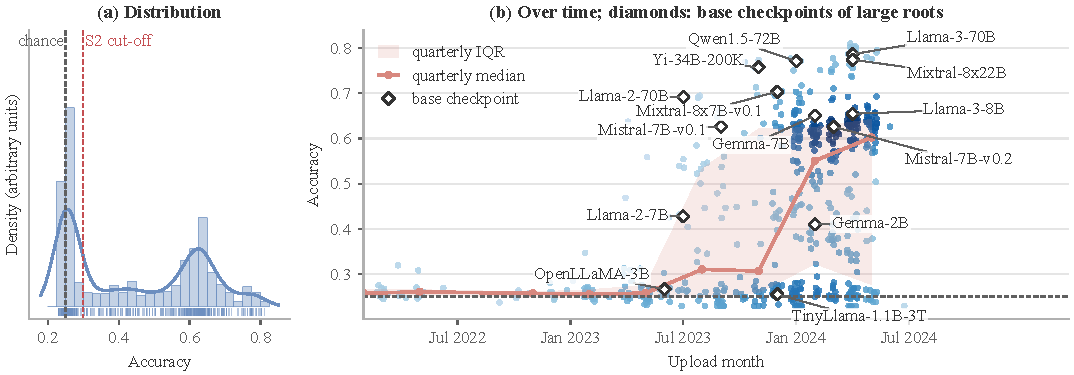
\includegraphics[width=0.65\textwidth]{fig_accuracy.pdf}
\caption{\textbf{Model accuracy} (primary sample, 590 models). (a) Histogram, kernel density and rug of the 590 accuracies; dashed lines mark chance for four options (0.25) and the S2 cut-off (0.30). (b) Accuracy by upload month (points shaded by local density, jittered within the month), with the median and interquartile range of each quarter containing at least 10 models; $\rho$: Spearman rank correlation between upload month and accuracy.}
\label{fig:accuracy}
\end{figure}

\begin{figure}[!htbp]
\centering
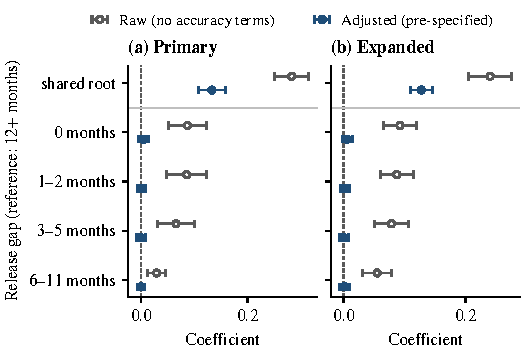
\includegraphics[width=\textwidth]{fig_raw_adjusted.pdf}
\caption{\textbf{Why accuracy must be adjusted for.} (a) All 173{,}755 primary pairs: agreement on wrong answers against the mean accuracy of the two models (hexagons: different-root pairs, log count; points: same-root pairs; lines: means in accuracy bins of 0.025 with at least 30 pairs; $r$: Pearson correlation). Agreement rises with accuracy, and same-root pairs are concentrated among accurate models. (b, c) Coefficients without (open) and with (filled) the accuracy terms; arrows show the change, and the lines above and below each marker are delete-one-root jackknife 95\% CIs. Release-gap bins are relative to 12 or more months. Adding the accuracy terms halves the shared-root coefficient and removes the graded release-gap association in both populations.}
\label{fig:rawadj}
\end{figure}

\subsection{Release Timing in Detail}
\label{sec:timing}
RQ2 asks whether release proximity is associated with agreement at equal lineage and accuracy. Fig.~\ref{fig:timing} shows every release-gap coefficient under the two timing measures. With upload months, all four gap bins are within 0.6 points of zero in both populations. With the roots' release months---closer to when the base model's data were assembled, and 12{,}271 different-root primary pairs have roots released in the same month---the coefficients are again near zero: $-0.1$ points for the same month (CI $-1.2$ to $+1.0$) in the primary sample, $+0.9$ (CI $-0.4$ to $+2.2$) in the expanded sample, and negative among models above 0.30 accuracy ($-2.2$, CI $-4.0$ to $-0.4$). Neither measure alone shows a positive association. Entered together, they split in the primary sample: same upload month $+1.8$ points (CI $+0.3$ to $+3.3$) and same root release month $-1.5$ ($-3.0$ to $-0.1$); in the expanded sample both are small ($+0.7$ and $+0.5$, intervals including zero), and among models above 0.30 accuracy $+1.3$ and $-3.3$ (Supplementary Section~S4). The two measures are correlated, so their coefficients partly offset each other.

Because this is an absence of evidence, we bound it. The 90\% jackknife interval for the pre-specified same-month coefficient excludes associations larger than 1.1 points in the primary sample and 1.3 points in the expanded sample, and 2.0--2.8 points among models above 0.30 accuracy, against 13.3 points for lineage. These bounds were not specified in advance. Release proximity may relate weakly to \emph{which items} fail together: the phi coefficient of error indicators and a CAPA-style agreement over all items show small positive same-month associations ($+0.018$ and $+0.013$ on their own scales), and excess co-failure over a Rasch model shows $+0.0036$ per item; the CAPA and Rasch versions disappear among models above 0.30 accuracy. Taken together, same-month pairs agree slightly more in several specifications---the option-distribution control S1 ($+1.0$), weighting by jointly wrong items ($+1.2$), accuracy-matched pairs ($+3.3$), the joint timing model ($+1.8$)---and less among models above 0.30 accuracy ($-1.5$ to $-2.2$). Release proximity is therefore associated with agreement on wrong answers at most weakly, with a sign that depends on the specification and a size well below the lineage difference.

\begin{figure}[!htbp]
\centering
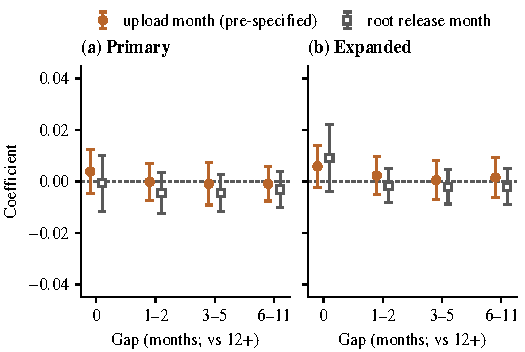
\includegraphics[width=0.65\textwidth]{fig_timing.pdf}
\caption{\textbf{Release-gap coefficients under two timing measures} (pre-specified model with accuracy terms; delete-one-root jackknife 95\% CIs). Upload month: the Hub creation month of each fine-tune. Root release month: that of its lineage root. Each bin is relative to a gap of 12 or more months.}
\label{fig:timing}
\end{figure}

\subsection{Robustness}
\label{sec:robust}
Table~\ref{tab:robust} collects every robustness check for the primary sample; detailed tables for all samples are in Supplementary Sections~S4 and S6.

\textbf{Inference.} Fig.~\ref{fig:inference} compares the three variance estimators in all four samples. Root-level procedures widen the shared-root interval by 10--26\% (root-level dyadic) and 39--63\% (jackknife), and every interval stays above 0.09. Only the S2 same-month coefficient changes conclusion: its jackknife interval includes zero. The jackknife relies on 63 roots with two or more models in the primary sample (108 in the expanded), and the two largest roots supply 1{,}407 of the 2{,}020 primary same-root pairs. Two further post-hoc procedures do not rest on asymptotic approximations (Supplementary Section~S6): a cluster bootstrap over roots gives a percentile interval of 11.4--19.6 points for the shared-root coefficient (expanded: 10.6--16.2), and shuffling root labels among models uploaded in the same quarter never produced a coefficient above 1.2 points in 999 permutations ($p = 0.001$, the smallest attainable).

\textbf{Item difficulty.} Conditioning on items both models get wrong compares strong pairs on harder items than weak pairs. A pair $\times$ item model with a fixed effect for each item, fitted over every pair and jointly wrong item (post hoc; Supplementary Section~S6), gives a shared-root coefficient of 14.2 points (jackknife CI 10.7--17.6), the same as the identically weighted pair-level fit without item effects, so the items on which a pair fails do not drive the contrast. Its same-month coefficient is $+1.1$ points ($-0.1$ to $+2.4$; expanded $+1.1$, 0.1--2.2), consistent with the weighted fit in Table~\ref{tab:robust}.

\begin{figure}[!htbp]
\centering
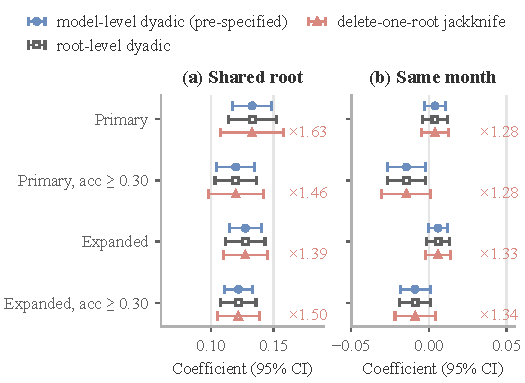
\includegraphics[width=0.65\textwidth]{fig_inference.pdf}
\caption{\textbf{Sensitivity of the intervals to the unit of dependence} (95\% CIs). Model-level dyadic: pairs sharing a model may be correlated (pre-specified). Root-level dyadic: pairs touching a common root may be correlated. Jackknife: one root, and every pair involving it, omitted at a time. Numbers: width of the jackknife interval relative to the model-level interval.}
\label{fig:inference}
\end{figure}

\textbf{Outcome definition.} Weighting pairs by their number of jointly wrong items (weighted least squares, WLS) gives 14.2 points for lineage. Subtracting the agreement expected from each model's distribution over answer options gives 12.5 points. The phi coefficient and the CAPA-style agreement, which also count whether the same items fail, show lineage associations of 0.170 and 0.194 on their own scales (a correlation and a kappa-type index, not percentage points).

\textbf{Item-difficulty-aware nulls.} With the nulls of Section~\ref{sec:defs}, the \emph{average} outcome falls from 0.423 to 0.002 (N1a) and 0.019 (N1b). For N1a this is close to zero largely by construction, because the null is computed from the same models, so it is not evidence about how much agreement popularity explains; the informative check is whether the lineage \emph{contrast} moves, and it is unchanged at 13.3 points (Fig.~\ref{fig:itemnull}), and changes by less than 0.2 points in every sample. The nulls shift related and unrelated pairs almost equally.

\begin{figure}[!htbp]
\centering
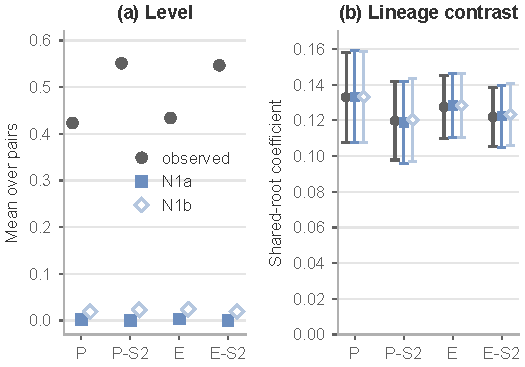
\includegraphics[width=0.65\textwidth]{fig_item_null_main.pdf}
\caption{\textbf{Shared-root coefficient under item-difficulty-aware nulls} (delete-one-root jackknife 95\% CIs): observed agreement, and agreement in excess of the item-level distractor null (N1a, all models; N1b, roots weighted equally). P: primary; E: expanded; S2: accuracy $\geq 0.30$. Mean outcome levels are in Supplementary Section~S4.}
\label{fig:itemnull}
\end{figure}

\textbf{Accuracy specification.} Agreement need not be linear in the two accuracies, and accuracy clusters within roots and upload months, so a misspecified accuracy control could bias both coefficients (post hoc; Supplementary Section~S6). With a full quadratic accuracy surface the shared-root coefficient is 12.3 points (jackknife CI 9.4--15.3); with a fixed effect for every pair of accuracy deciles, 12.7; with 20 accuracy bins (210 cells), 11.9 (8.5--15.3); and among the 28{,}170 pairs whose accuracies differ by at most 0.02, 14.8 (10.7--18.9). Across the four samples these specifications give 11.0 to 14.9 points. Without any accuracy terms the coefficient is 28.3 points, so about half of the raw lineage contrast runs through accuracy (Fig.~\ref{fig:rawadj}). Under the flexible controls the same-month coefficient lies between $-1.2$ and $+0.6$ points in every sample, but among accuracy-matched pairs it is $+3.3$ points (1.4--5.2) in the primary sample and $+3.4$ to $+5.6$ points in the others, with an interval excluding zero in three of the four. Same-month pairs of nearly equal accuracy therefore agree somewhat more; whether that reflects a shared era or accuracy structure finer than the matching removes, the data cannot say.

\textbf{Controls, timing measure and data quality.} Adding model size and a same-architecture indicator leaves 12.6 points; lineage and architecture are nested here, so this partitions one association. Measuring release timing by the roots' release months leaves the lineage coefficient at 13.1 points (Section~\ref{sec:timing}). Removing the degenerate models and collapsing identical-prediction clusters gives 12.8 points; keeping only models whose configuration file agrees with their declared root gives 13.5; the cap-15 subset of the sample gives 14.6. Removing the 369 items that MMLU-Redux 2.0~\cite{gema2025} annotates as erroneous, among the 5{,}698 of our items it re-annotates, leaves 13.4 points, and the 5{,}329 items it annotates as correct give 13.3 (post hoc; Supplementary Section~S6), so answer-key errors do not drive the estimate.

\textbf{Independent check of lineage.} For 191 primary models, the configuration file names another Hub repository; following that link reaches the declared root in 142 cases (74\%), another root in 48 and none in 1. The disagreements mix declaration errors, such as continued-pretraining models declared as their own roots, with configuration files copied from other models.

\begin{table}[!htbp]
\caption{\textbf{Robustness checks} (primary sample; 95\% CIs from the SE type shown). Same month: 0-month gap bin relative to 12 or more months. $^{a}$Different outcome scale (correlation, chance-adjusted agreement or co-failure per item). Plan, run late: in the analysis plan but run after review. $^{b}$Tree distance replaces the shared-root indicator: the number of declared links between the two models through their nearest common ancestor.}
\label{tab:robust}
\centering
\footnotesize
\resizebox{\ifdim\width>\textwidth\textwidth\else\width\fi}{!}{\begin{tabular}{llccc}
\toprule
Check & Status & SE & Shared root & Same month \\
\midrule
\tabinput{../../paper/tables/tab_robust.tex}
\bottomrule
\end{tabular}}
\end{table}

\subsection{Lineage Dose-Response}
If shared errors are inherited, closer relatives should agree more. The tree-distance predictor was specified in the analysis plan as secondary but first run after review, when the main results were known, so we treat it as supporting rather than confirmatory evidence. Replacing the shared-root indicator by tree distance gives a monotone gradient (Table~\ref{tab:robust}): 18.5 points for parent--child pairs (177 pairs), 13.6 at distance two (699, mostly siblings) and 11.5 for more distant relatives (1{,}112). Classified by relation, ancestor--descendant pairs agree 17.3 points more than unrelated pairs, siblings 13.5 and more distant relatives 11.5 (Fig.~\ref{fig:dose}). The 32 same-root pairs at distance zero, one Hub repository listed under two leaderboard names, have their own indicator and are not shown. Parent--child pairs come disproportionately from small roots (82 of 177), which show larger coefficients (Section~\ref{sec:hetero}), so the gradient could reflect root composition. Estimated within roots (post hoc; same-root pairs only, with a fixed effect for each root), parent--child pairs agree 5.5 points more than distance-3+ pairs of the same root (jackknife CI 4.1--6.8) and distance-two pairs 2.3 points more (0.3--4.2); the gradient is smaller within roots than across them, but present. Closer relatives are also uploaded closer together and often by the same developer, so the gradient is consistent with inheritance but does not isolate it.

\begin{figure}[!htbp]
\centering
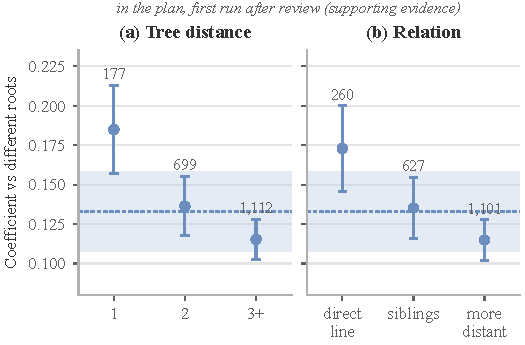
\includegraphics[width=0.65\textwidth]{fig_dose.pdf}
\caption{\textbf{Lineage dose-response} (primary sample; in the analysis plan, run after review; delete-one-root jackknife 95\% CIs; labels: number of pairs). Each coefficient compares one kind of related pair with pairs from different roots, in the pre-specified model with the shared-root indicator replaced. Tree distance: declared links between the two models through their nearest common ancestor; the 32 pairs at distance zero (one repository under two names) have their own indicator and are not shown. Shaded band and dashed line: the pre-specified shared-root coefficient and its interval.}
\label{fig:dose}
\end{figure}

\subsection{Where the Lineage Association Comes From}
\label{sec:hetero}
The contrast is identified by 63 roots, two of which contribute 39 and 37 models, so we examined how it is spread (Fig.~\ref{fig:heterogeneity}). \emph{By root}, each of the seven roots with at least eight models shows its own shared-root coefficient, from 10.3 points (Gemma-7B) to 14.8 (Gemma-2B), every interval excluding zero; the 56 smaller multi-model roots together show 22.0 points, and 19.8 after removing duplicate and degenerate models. That is consistent with the dose-response result, since small roots are often a single developer's successive versions, but we did not test it directly. Dropping any single root, with every pair involving it, leaves the primary estimate between 13.1 and 14.4 points. The pre-specified coefficient weights roots by their number of same-root pairs, so the two largest roots, which supply 1{,}407 of the 2{,}020 same-root pairs and have among the smallest coefficients, dominate it. Counting each root once gives a larger estimate (post hoc; Supplementary Section~S6): the unweighted mean of the 63 per-root coefficients is 25.3 points, and a random-effects pooling of the 16 roots with at least 10 same-root pairs gives 16.6 points (CI 12.5--20.8; between-root standard deviation 7.9 points). The 13.3 points therefore describe the population as sampled, not a typical root. \emph{By capability}, the coefficient is 13.3 points among pairs whose weaker model scores at least 0.60 and 11.6 at 0.50--0.60; below 0.50 the few same-root pairs give imprecise estimates. \emph{By subject}, the coefficient is positive with a model-level interval excluding zero in all 57 MMLU subjects, with a median of 12.2 points and a range from 7.0 (management) to 18.0 (moral scenarios). The same analysis gives a median same-month coefficient of $+0.6$ points across subjects, with model-level intervals excluding zero in 13 subjects, 12 of them positive. That is more than the roughly three expected by chance, so a small positive release-proximity association in some subjects cannot be excluded, although model-level intervals tend to be too narrow here.

\begin{figure}[!htbp]
\centering
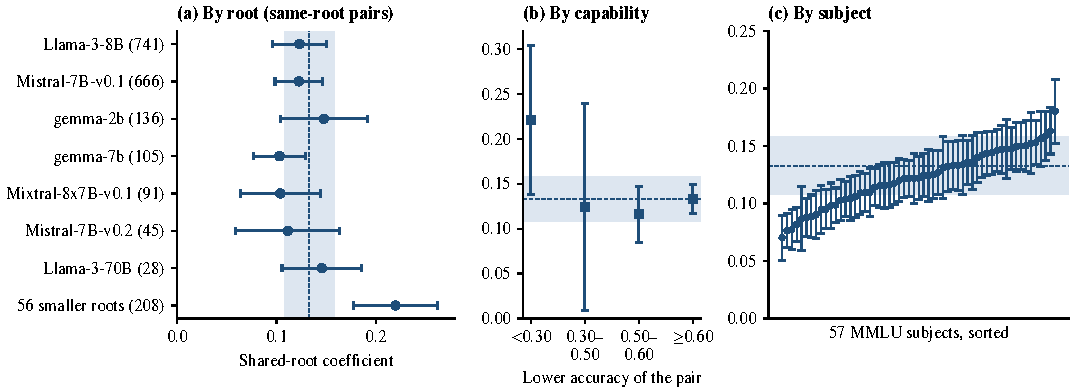
\includegraphics[width=\textwidth]{fig_heterogeneity.pdf}
\caption{\textbf{Heterogeneity of the lineage association} (primary sample; post hoc). (a) Shared-root coefficient for each root with at least eight models and for the remaining multi-model roots pooled (labels and marker area: same-root pairs; model-level dyadic 95\% CIs, since a jackknife over roots is undefined for a single root). (b) By the lower accuracy of the two models (jackknife 95\% CIs). (c) For each of the 57 MMLU subjects, with the outcome computed on that subject's items (model-level 95\% CIs, which tend to be too narrow; 57 tests without multiplicity adjustment), coloured by the MMLU category of the subject as tagged in the LM Evaluation Harness. Shaded band and dashed line: the pre-specified estimate and its jackknife interval.}
\label{fig:heterogeneity}
\end{figure}

An exploratory analysis of how well agreement separates same-root from different-root pairs is in Supplementary Section~S5; it is descriptive and not a validated lineage detector.

\section{Discussion}
\label{sec:discussion}

\textbf{What the results say.} In this population, which base model a fine-tune descends from is strongly associated with which wrong answers it gives: related pairs agree on wrong answers about 13 points more often, a 31\% increase over the mean, and, in an analysis run after review, more the closer the relation. When a model was released matters at most weakly once accuracies are known: same-month associations are a few points or less, and their sign depends on the specification. This is consistent with Kim~\textit{et al.}'s finding that shared provider and architecture predict agreement~\cite{kim2025}, and adds that, with lineage taken from declared ancestry and timing measured directly, the association in this population is tied to lineage far more than to release proximity.

\textbf{What they do not say.} The association is observational. Fine-tunes of one base share its parameters, its pretraining data and often similar post-training data; the design does not separate these routes or show that fine-tuning causes inherited errors. Nor does it show that release timing is irrelevant: the pretraining era of a base model is shared by its fine-tunes and therefore nested in lineage here, contemporaneous models agree more partly because they are similarly accurate, and timing may relate weakly to which items fail together.

\textbf{Why lineage and not release timing.} A fine-tune starts from its base model's weights and is typically trained on far less data than its base; much of the base model's knowledge, and its gaps, plausibly survive. Three features of the results, all from analyses run after review, fit this reading: the association grows with closeness of descent, it is present in every MMLU subject rather than concentrated in a few, and it survives nulls that account for which distractors are attractive on each item, so it is not explained by related models simply finding the same items hard. Models uploaded in the same month share only what was common at the time---popular base models, datasets and recipes---and in this population that commonality is largely captured by lineage and accuracy. These are hypotheses consistent with the results, not mechanisms the design tests; distinguishing inherited weights from shared fine-tuning data would require models fine-tuned from one base on controlled data.

\textbf{How far the results generalize.} The population is the first Open LLM Leaderboard: open-weight models, mostly community fine-tunes of a few dozen bases released from 2022 to 2024, evaluated by log-likelihood on four-option questions. Within these data the lineage result is consistent across re-analyses---every large root, every subject, model capability above 0.50 accuracy, and outcomes that measure which items fail as well as which option is chosen---but these are post-hoc analyses of the same observations, not replications, and say little about other populations. Two features limit the timing result: pretraining eras are nested in lineage here, and the period spans only 27 months. Closed models, generative tasks scored by judges, and populations of independently pretrained models could all behave differently.

\textbf{Relation to earlier evidence.} Kim~\textit{et al.}~\cite{kim2025} found that a shared provider and shared base architecture predict agreement; resolving lineage per model shows that descent from the same declared checkpoint is associated with agreement at equal accuracy and, in an analysis run after review, that the association grows with closeness of descent. Provider was not controlled, and architecture is nested in lineage here, so the two explanations are not separated. Goel~\textit{et al.}~\cite{goel2025} report that mistakes become more similar as capability rises; our accuracy-sum coefficient is positive, consistent with this, and the unadjusted release-time gradient is what such a capability trend would produce in a population whose models improved over time. Jo~\textit{et al.}~\cite{jo2026} warn that levels of excess agreement depend on the null; our item-level nulls confirm this for levels and show that the lineage contrast does not depend on it.

\textbf{What the numbers mean for model selection.} When two fine-tunes of one base both fail an item, they choose the same wrong option about three times in four; two models from different roots do so about two times in five. A reviewer or ensemble that treats agreement between two related models as independent confirmation therefore over-counts it more than it would for unrelated models. Release timing, net of accuracy, offers at most a weak and specification-dependent signal in these data; whether choosing models from different periods would change their agreement on wrong options is a question about intervention that this observational design does not answer.

\textbf{What would change these conclusions.} Three findings would weaken them: a lineage contrast that vanishes on other benchmarks or evaluation pipelines; lineage inferred from weights that disagrees with declarations often enough to reverse the dose-response; and, among independently pretrained models released at the same time, a release-time association that the present population cannot show because its pretraining eras are nested in lineage.

\textbf{Recommendations for leaderboards and model hubs.} Three practices would make studies like this one easier and more reliable. Leaderboards could record a canonical repository identifier, since renamed repositories left 50 primary entries pointing to 23 models. They could flag degenerate outputs, such as the 21 primary models that answer one letter on almost every item. And hubs could encourage machine-readable parent declarations: 70\% of leaderboard models declare none, which limits any lineage analysis to a documented minority.

\textbf{Implications.} The results suggest, as a hypothesis for practitioners, that drawing ensemble members from different base models may reduce shared wrong answers more than drawing them from one base at different times. We did not test this. The effect on ensemble accuracy depends on how members are combined~\cite{chen2026}, and capability-controlled audits find that shared errors predict majority-vote gain only modestly~\cite{kimd2026}.

\section{Limitations}
\label{sec:limitations}
\begin{enumerate}
\item \textbf{Population and design.} The associations are observational, in a self-selected population dominated by community fine-tunes of a few dozen bases from 2022 to 2024. They may not hold for frontier or closed models, or for separately pretrained models released at the same time.
\item \textbf{Lineage measurement.} Declared parents can be wrong or missing. Random misclassification would bias the lineage contrast towards zero; misclassification related to how models err could bias it either way. Excluding undeclared models shifts the population towards documented fine-tunes. Estimates agree across the primary, expanded and strict populations (12.7--13.4 points) and in config-consistent models, but lineage was not verified from weights.
\item \textbf{Release-timing measurement.} Upload and root release months are proxies for when training data were assembled, and for same-root pairs the pretraining era is shared by construction, so pretraining era cannot be separated from lineage. The Hub creation month is also a noisy measure of when a model was built; such noise biases release-time coefficients towards zero, so the equivalence bounds are looser than they appear.
\item \textbf{Benchmark and pipeline.} One benchmark with four options is used, and all predictions come from the leaderboard's evaluation pipeline. Model-specific configuration errors cannot be ruled out; 339 of 977 models score below 0.30, which the S1 and S2 analyses address only in part. Contamination could make agreement partly reflect shared memorization. Removing the items that MMLU-Redux annotates as erroneous does not change the estimate, but that check covers 5{,}698 of the 14{,}042 items.
\item \textbf{Outcome scope.} The outcome counts only items both models get wrong; it is not a measure of ensemble performance, and its level depends on the null model and population~\cite{jo2026}.
\item \textbf{Identification.} Same-root pairs are almost all within a year of each other, so the data cannot show whether the lineage association persists between fine-tunes released far apart. The contrast comes from 63 roots, two of which contribute 39 and 37 models, although every large root shows it separately and no single root changes it by more than 1.1 points. Because the estimate weights roots by their number of pairs, it is smaller than the average over roots (Section~\ref{sec:hetero}).
\item \textbf{Design check and plan.} The simulation check narrowly missed its leakage criterion at the strongest simulated release-time effect, and model-level SEs were 3--5\% too small in simulation; we therefore report root-level intervals. With the real accuracies, a non-linear dependence of agreement on ability inflated false rejection under the linear accuracy control, which is why flexible controls are reported. The analysis plan was not registered externally, its timing rests on the repository's commit times within a single day, and several analyses are post hoc (Table~\ref{tab:status}).
\end{enumerate}

\section{Conclusion}
\label{sec:conclusion}
Among open-weight models on the first Open LLM Leaderboard, two models that share a declared lineage root choose the same wrong MMLU option, when both are wrong, about 13 percentage points more often than unrelated models of equal accuracy and release gap; an analysis run after review suggests that closer relatives agree more. The estimate is stable across the analyses fixed in advance, root-level inference, alternative outcomes, item-difficulty-aware nulls and cleaned samples. Net of accuracy, release proximity---of the models or of their base models---is associated with the choice of wrong option at most weakly: a few points or less, with a sign that depends on the specification. The next step is to test whether lineage diversity improves ensemble, voting or review performance on other benchmarks, evaluation pipelines and independently pretrained models.

\section*{Appendix: Earlier Per-Model Evaluation---Model Roster, Execution Environment and Data-Integrity Audit}
\label{app:runpod}
This appendix summarizes the earlier per-model evaluation mentioned in the Introduction; Supplementary Section~S7 gives the full record. None of its measurements is used in this paper, and it does not validate any result reported here. Of 20 planned evaluations, 16 were run before the work was stopped for budget reasons; the two DeepSeek entries of the 22-entry roster were to be completed by imputation, which was never executed. Table~\ref{tab:runpodmain} lists every planned entry, and Table~\ref{tab:runpodenv} gives the execution environment with the evidence for each item. Every recorded per-question file fails the intake check: it stores one log-likelihood per item and predicts option~A on all 14{,}042 items, because the extraction code read only the first option's score. The recorded accuracies are \texttt{lm-eval}'s own aggregates and are not validated item by item; several are at chance level for reasons not established.

\begin{sidewaystable}
\caption{\textbf{Earlier per-model evaluation: planned roster, execution and data status} (not used for inference). Repository: the repository actually evaluated, or the planned one where no run exists. Size: as planned, and as named by the recorded repository where it differs. Planned: precision in the frozen run plan. Recorded: precision tag in the result file. Data: outcome of the intake check on the per-question file. Note: \texttt{lm-eval} aggregate accuracy flags and, where the same repository is in the item-validated leaderboard data of this paper, its accuracy there. $^{a}$Repository differs from the plan. $^{b}$Tag written by the run script; the 4-bit path selects the \texttt{bitsandbytes} default type (FP4, not the planned NF4), and a loader patch removed quantization arguments for one Mistral model class, so the precision actually used is not confirmed. $^{c}$One log-likelihood per item and a constant prediction (option A). $^{d}$Planned repository; no run exists.}
\label{tab:runpodmain}
\centering
\footnotesize
\setlength{\tabcolsep}{2pt}
\resizebox{\ifdim\width>\textheight\textheight\else\width\fi}{!}{%
\begin{tabular}{llllllllp{0.2\textheight}}
\toprule
Model & Family & Repository & Size & Planned & Recorded & Execution & Data & Note \\
\midrule
\tabinput{../../paper/tables/tab_runpod_main.tex}
\bottomrule
\end{tabular}}
\end{sidewaystable}

\begin{table}[!htbp]
\caption{\textbf{Execution environment of the earlier per-model evaluation and the evidence for each item.} Recorded after run: stated in the project's reproducibility checklist of 19 August 2026, written after the runs; no pod log survives. Planned: stated in the run plan of 16 August 2026, before the first run. Author-reported: supplied by the authors; no record in the repository. Unknown: no record.}
\label{tab:runpodenv}
\centering
\scriptsize
\setlength{\tabcolsep}{3pt}
\resizebox{\ifdim\width>\textwidth\textwidth\else\width\fi}{!}{\begin{tabular}{p{0.17\textwidth}p{0.36\textwidth}p{0.13\textwidth}p{0.26\textwidth}}
\toprule
Item & Value & Status & Source \\
\midrule
Provider and GPU & RunPod; one NVIDIA A100-SXM4, 80\,GB; one GPU, not a cluster & Recorded after run & Reproducibility checklist; run plan \\
Host CPU and RAM & 16 vCPUs; 117\,GB RAM & Author-reported & -- \\
Disk & At least 300\,GB GPU disk planned (70B weights downloaded in bfloat16 before 4-bit loading); actual attached storage not known & Planned only & Run plan \\
Python & 3.11 (PyTorch template) & Planned only & Run plan \\
PyTorch & 2.8.0 (pod template) & Author-reported & -- \\
\texttt{lm-eval} & 0.4.12 & Planned; supported & Run plan; code fixes for the 0.4.12 output format made during the run \\
\texttt{transformers} & 4.57.6 (pinned because version 5 removed the \texttt{load\_in\_4bit} argument) & Planned only & Run plan; pin committed before the first run \\
\texttt{accelerate}, \texttt{bitsandbytes} & Installed, versions not pinned & Unknown version & Run plan \\
Task and intended scoring & MMLU, 5-shot, log-likelihood scoring of the four answer options; 14{,}042 items per model. The saved per-question extraction is invalid and keeps one score per item, not the four option-level scores & Planned; items recorded & Run plan; result files (14{,}042 rows each) \\
Model arguments & \texttt{dtype=bfloat16}, \texttt{attn\_implementation=sdpa}, automatic batch size; \texttt{load\_in\_4bit=True} for 4-bit runs; \texttt{max\_length=2048}, truncation for Phi-1, Phi-1.5, Phi-2 & Planned; in code & Run plan; run script (\texttt{phase2\_eval.py}) \\
Run time & Not measured; commits of results span 16 Aug 18:08 to 18 Aug 09:12 UTC (wall-clock, including idle time) & Unknown & Commit history \\
Cost & Estimated USD 16--20 for the full plan at about USD 1.60/h; amount billed not known & Planned only & Run plan \\
Intake check & Fails: 4 planned models missing, \texttt{acc\_norm} empty, all 16 per-question files invalid & Verified & Check run on the committed files, 10 Oct 2026 \\
\bottomrule
\end{tabular}}
\end{table}

\section*{Data Availability}
{\sloppy
Code, frozen model lists with SHA-256 hashes, Hugging Face metadata caches, validation reports and all analysis outputs are available at \url{https://github.com/Sudharsanselvaraj/Identifiable-Variance-Decomposition-of-Correlated-Errors-in-Foundation-Models}; the README lists the commands that regenerate every reported number, table and figure from these outputs. The leaderboard's per-item details and metadata declare no licence, so the derived item-level answer files and three copied metadata fields are not redistributed; released scripts regenerate them from the public source and verify them against the recorded hashes. The analysis plan and its amendments are in the repository, as are the records of the earlier per-model evaluation (Appendix; Supplementary Section~S7), which are not used for inference. Supplementary material accompanies this article.\par}

\section*{Acknowledgment}
This work was supported in part by the Department of Computer Science and Engineering, SRM Institute of Science and Technology, Tiruchirappalli, India, and in part by the Research Institute of IoT Cybersecurity, National Kaohsiung University of Science and Technology, Kaohsiung, Taiwan.

\textbf{Use of AI-generated content.} The authors used Claude (Anthropic; model Claude Opus 5.5, accessed through Claude Code)~\cite{claude2026} in October 2026, with substantial use. It wrote and debugged the analysis, simulation, data-extraction and figure/table-generation code, and drafted the text of every section of this revised manuscript (Sections~\ref{sec:introduction}--\ref{sec:conclusion}) and of the supplementary material. The authors directed the study, approved each analysis decision and analysis-plan amendment, reviewed and edited the text, and take full responsibility for the content; every reported number is produced by the released code from the committed outputs.

\begin{thebibliography}{40}

\bibitem{kim2025} E.~Kim, A.~Garg, K.~Peng, and N.~Garg, ``Correlated errors in
large language models,'' in \emph{Proc. Int. Conf. Mach. Learn. (ICML)},
vol.~267, pp.~30038--30066, 2025.

\bibitem{dietterich2000} T.~G.~Dietterich, ``Ensemble methods in machine
learning,'' in \emph{Proc. Int. Workshop Multiple Classifier Syst.}, LNCS 1857,
2000, pp.~1--15.

\bibitem{kuncheva2003} L.~I.~Kuncheva and C.~J.~Whitaker, ``Measures of
diversity in classifier ensembles and their relationship with the ensemble
accuracy,'' \emph{Mach. Learn.}, vol.~51, no.~2, pp.~181--207, 2003.

\bibitem{chen2026} J.~L.~Chen, ``When does combining language models help? A
co-failure ceiling on routing, voting, and mixture-of-agents across 67 frontier
models,'' \emph{arXiv preprint arXiv:2606.27288}, 2026.

\bibitem{kuai2026} C.~Kuai \emph{et al.}, ``A statistical framework for auditing
behavioral dependence and induced bias in LLM judges,'' \emph{arXiv preprint
arXiv:2604.07650v2}, 2026.

\bibitem{goel2025} S.~Goel, J.~Str\"uber, I.~A.~Auzina, K.~K.~Chandra,
P.~Kumaraguru, D.~Kiela, A.~Prabhu, M.~Bethge, and J.~Geiping, ``Great models
think alike and this undermines AI oversight,'' in \emph{Proc. Int. Conf. Mach.
Learn. (ICML)}, vol.~267, pp.~19621--19678, 2025.

\bibitem{kimd2026} D.~Kim, ``Are diversity metrics measuring diversity? A
capability-controlled audit of majority-vote gain in LLM ensembles,''
\emph{arXiv preprint arXiv:2607.20768}, 2026.

\bibitem{bugaud2026} Z.~Bugaud, ``Hidden clones: Exposing and fixing family bias
in vision-language model ensembles,'' \emph{arXiv preprint arXiv:2603.17111}, 2026.

\bibitem{lihai2026} H.~Li and M.~Hai, ``State-dependent error correlations shape
voting thresholds in committees of AI agents,'' \emph{arXiv preprint
arXiv:2607.23931}, 2026.

\bibitem{hossain2026} E.~Hossain \emph{et al.}, ``Right knowledge, wrong answer:
Characterizing parametric temporal conflict in open-weight language models,''
\emph{arXiv preprint arXiv:2606.20959}, 2026.

\bibitem{tieman2026} R.~Tieman and E.~Markou, ``Inferred generative-process
diversity predicts correlated failure across language models,'' \emph{arXiv
preprint arXiv:2609.03422}, 2026.

\bibitem{jo2026} N.~Jo, N.~Garg, and M.~Raghavan, ``The subjectivity of
monoculture,'' \emph{arXiv preprint arXiv:2602.24086}, 2026.

\bibitem{laufer2025} B.~Laufer, H.~Oderinwale, and J.~Kleinberg, ``Anatomy of a
machine learning ecosystem: 2 million models on Hugging Face,'' \emph{arXiv
preprint arXiv:2508.06811}, 2025.

\bibitem{horwitz2025} E.~Horwitz, A.~Shul, and Y.~Hoshen, ``Unsupervised model
tree heritage recovery,'' in \emph{Proc. Int. Conf. Learn. Represent. (ICLR)},
2025.

\bibitem{wu2026dna} Z.~Wu, H.~Zhao, Z.~Wang, J.~Guo, Q.~Wang, and B.~He, ``LLM
DNA: Tracing model evolution via functional representations,'' in \emph{Proc.
Int. Conf. Learn. Represent. (ICLR)}, 2026.

\bibitem{tamura2025} T.~Tamura, T.~Yano, M.~Enomoto, and M.~Oyamada, ``Can a crow
hatch a falcon? Lineage matters in predicting large language model
performance,'' \emph{arXiv preprint arXiv:2504.19811}, 2025.

\bibitem{choi2026} M.~Choi \emph{et al.}, ``The truth stays in the family:
Enhancing contextual truthfulness via inherited heads in model lineages,''
in \emph{Proc. Int. Conf. Mach. Learn. (ICML)}, vol.~306, pp.~20021--20044, 2026.

\bibitem{nikolic2025} I.~Nikoli\'c, T.~Baluta, and P.~Saxena, ``Model provenance
testing for large language models,'' in \emph{Proc. Adv. Neural Inf. Process.
Syst. (NeurIPS)}, 2025.

\bibitem{phylolm2024} N.~Yax, P.-Y.~Oudeyer, and S.~Palminteri, ``PhyloLM:
Inferring the phylogeny of large language models and predicting their
performances in benchmarks,'' in \emph{Proc. Int. Conf. Learn. Represent.
(ICLR)}, 2025.

\bibitem{li2026roots} Y.~Li \emph{et al.}, ``Tracing the roots: A multi-agent
framework for uncovering data lineage in post-training LLMs,'' in \emph{Proc.
64th Annu. Meeting Assoc. Comput. Linguist. (Volume 1: Long Papers)}, 2026,
pp.~9606--9625.

\bibitem{patterson1971} H.~D.~Patterson and R.~Thompson, ``Recovery of
inter-block information when block sizes are unequal,'' \emph{Biometrika},
vol.~58, no.~3, pp.~545--554, 1971.

\bibitem{harville1977} D.~A.~Harville, ``Maximum likelihood approaches to variance
component estimation and to related problems,'' \emph{J. Amer. Statist. Assoc.},
vol.~72, no.~358, pp.~320--338, 1977.

\bibitem{searle1992} S.~R.~Searle, G.~Casella, and C.~E.~McCulloch,
\emph{Variance Components}. New York, NY, USA: Wiley, 1992.

\bibitem{brennan2001} R.~L.~Brennan, \emph{Generalizability Theory}. New York, NY,
USA: Springer, 2001.

\bibitem{messing2026} S.~Messing, ``Hidden measurement error in LLM pipelines
distorts annotation, evaluation, and benchmarking,'' \emph{arXiv preprint
arXiv:2604.11581}, 2026.

\bibitem{fafchamps2007} M.~Fafchamps and F.~Gubert, ``The formation of risk
sharing networks,'' \emph{J. Develop. Econ.}, vol.~83, no.~2, pp.~326--350, 2007.

\bibitem{cameron2011} A.~C.~Cameron, J.~B.~Gelbach, and D.~L.~Miller, ``Robust
inference with multiway clustering,'' \emph{J. Bus. Econ. Statist.}, vol.~29,
no.~2, pp.~238--249, 2011.

\bibitem{aronow2015} P.~M.~Aronow, C.~Samii, and V.~A.~Assenova,
``Cluster-robust variance estimation for dyadic data,'' \emph{Political Anal.},
vol.~23, no.~4, pp.~564--577, 2015.

\bibitem{efron1982} B.~Efron, \emph{The Jackknife, the Bootstrap and Other
Resampling Plans}. Philadelphia, PA, USA: SIAM, 1982.

\bibitem{breiman2001} L.~Breiman, ``Random forests,'' \emph{Mach. Learn.},
vol.~45, no.~1, pp.~5--32, 2001.

\bibitem{kleinberg2021} J.~Kleinberg and M.~Raghavan, ``Algorithmic monoculture
and social welfare,'' \emph{Proc. Nat. Acad. Sci. USA}, vol.~118, no.~22,
2021.

\bibitem{bommasani2022} R.~Bommasani, K.~A.~Creel, A.~Kumar, D.~Jurafsky, and
P.~Liang, ``Picking on the same person: Does algorithmic monoculture lead to
outcome homogenization?'' in \emph{Adv. Neural Inf. Process. Syst. (NeurIPS)},
vol.~35, 2022.

\bibitem{beeching2023} E.~Beeching \emph{et al.}, ``Open LLM Leaderboard
(2023--2024),'' Hugging Face, 2023. [Online]. Available:
\url{https://huggingface.co/spaces/open-llm-leaderboard-old/open_llm_leaderboard}

\bibitem{hendrycks2021} D.~Hendrycks \emph{et al.}, ``Measuring massive multitask
language understanding,'' in \emph{Proc. Int. Conf. Learn. Represent. (ICLR)},
2021.

\bibitem{gao2021} L.~Gao \emph{et al.}, ``A framework for few-shot language model
evaluation,'' Zenodo, 2021, doi: 10.5281/zenodo.5371628.

\bibitem{paquin2026} D.~Paquin and R.~Jain, ``What does MMLU actually measure? A
psychometric audit of difficulty structure in aggregate benchmark scores,''
\emph{arXiv preprint arXiv:2609.09372}, 2026.

\bibitem{gema2025} A.~P.~Gema \emph{et al.}, ``Are we done with MMLU?,'' in \emph{Proc. Conf. North Amer. Chapter Assoc. Comput. Linguistics (NAACL)}, 2025, pp.~5069--5096, doi: 10.18653/v1/2025.naacl-long.262.

\bibitem{claude2026} Anthropic, ``Claude (Claude Opus 5.5), accessed through
Claude Code,'' large language model, Oct. 2026. [Online]. Available:
\url{https://www.anthropic.com/claude}

\end{thebibliography}

\end{document}
